\documentclass[12pt]{article}
\usepackage[margin=1in]{geometry}
\usepackage{natbib}
\usepackage{graphicx}
\usepackage{subcaption}
\bibliographystyle{apalike}
\begin{document}

\title{Rare alleles and the genetic basis of crop phenotypes}
\date{}
\maketitle

Thinking about population demography and effects on genetic architecture of traits.

intro to quantitative traits

 understanding them is key

 traditionally, QTL has been used

 recently GWAS, potential to identify individual genes

 missing heritability

rare alleles of large negative effect often missed \citep{Thornton2013}


demographic effects can impact deleterious allele distro

$V_a$ influenced by demography \citep{Lohmueller2014}


These guys did crap \citep{Gazave2013}.
But \citet{Thornton2014} did more.


\begin{figure}
\centering
   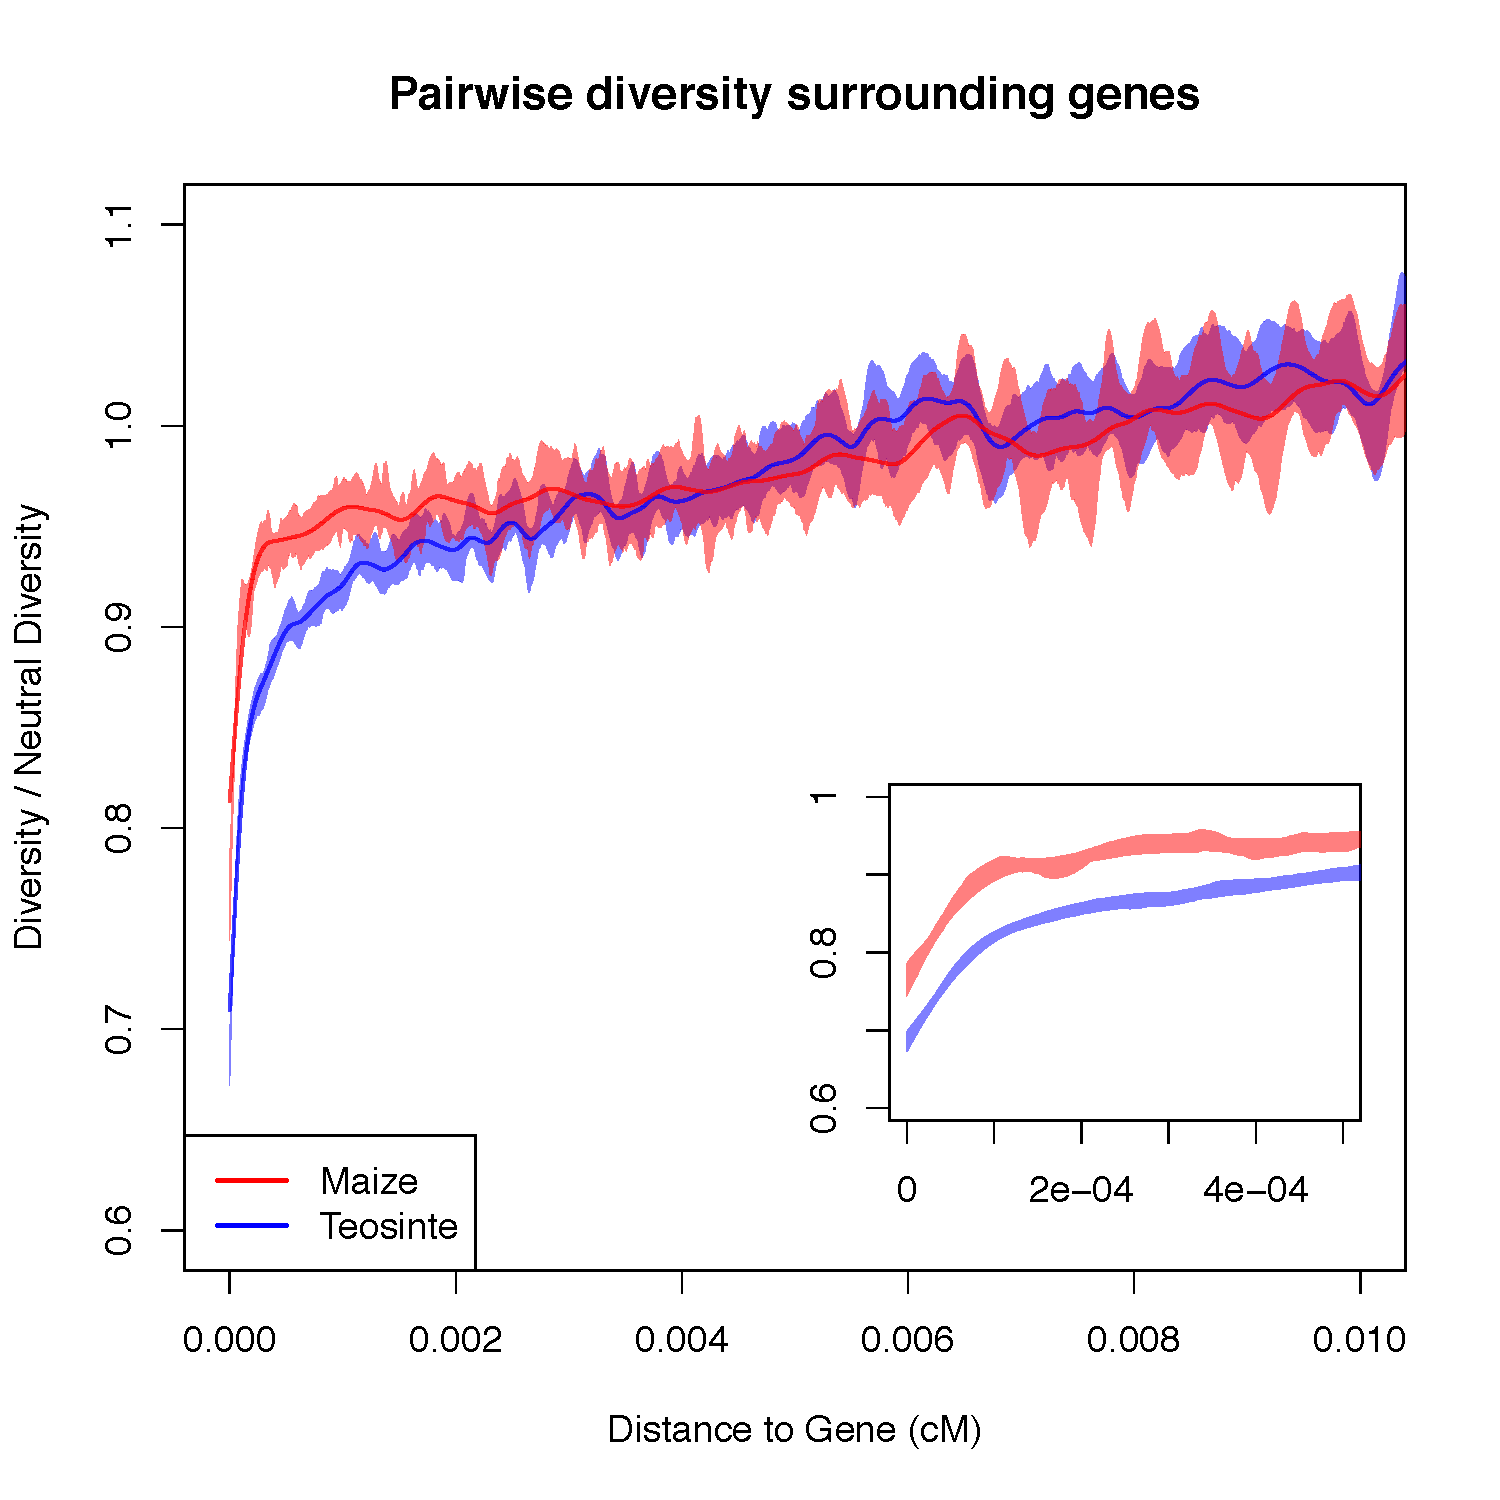
\includegraphics[width=0.8\textwidth]{pairwise.pdf}
  \caption{All polymorphisms}
  \label{fig:sub1}
\end{figure}%




For designing breeding strategies, for utilizing diversity from wild relatives, for understanding variation in phenotype, for engineering new traits (GMOs, CRISPR).




\bibliography{/Users/jri/Documents/references/references.bib}
\end{document}